\documentclass[a4paper]{article}
\usepackage[hidelinks]{hyperref}

\title{Architectural Design
\\COS 301 Buzz Project
\\Group 2A
\\Version 1.0}

\author{Goodness Adegbenro 13046412
\\Elzahn Botha 13033922
\\Carla de Beer 95151835
\\Sboniso Masilela 10416260
\\Mandla Mhlongo 29630135
\\Isabel Nel 13070305
\\Ndivhuwo Nthambeleni 10001183
\\Lutfiyya Razak 10198408
\\
\\
\url{https://github.com/Isabel01/COS-301-2a-Round-2}
\\
\\ University of Pretoria}

\date{11 March 2015}

% Need to compile using XeLATeX to avoid default font
%usepackage{fontspec}
%setmainfont{Arial}
% Graphics settings for .eps files
\usepackage{graphicx}
\usepackage{epstopdf}
\DeclareGraphicsExtensions{.eps}
\usepackage{float}

\begin{document}

\maketitle
% No page number to cover page
\pagenumbering{gobble}
\newpage
% start page numbering
\pagenumbering{arabic}

% Generate Table of Contents

\tableofcontents
\newpage

\section{Introduction}
<<<<<<< HEAD
t sets out the software architecture design requirements for the COS 301 group project entitled Buzz.
\\
\\In terms of a definition, software architecture can be defined as
\\
\\\textit{“... a system or subsystem [that] refers to the style of design of the structure of the system including the interfacing and interaction among its major components.”}
\\
\\And software architectural design, in turn, can be defined as
\\
\\\textit{“ ... a decision-making process to determine the software architecture for the system under development”} (KUNG, 2014, p140).
\\
\\Thus, software architecture deals as much with the design of a software system as with the decision-making process involved in determining the most optimal architectural design.
High-level architectural patterns, or styles, are often associated with the architectural design process, patterns such as layered architecture, component-based architecture, model-view-controller, and the pipes and filters pattern (MICROSOFT DEVELOPER NETWORK, n.d.).
=======
rala's intro goes here.....

The idea behind the 'Buzz' project is to find ways to enhance teaching and improve the learning of students through the use of online discussions. The 'Buzz' will be an online forum where students can express their views on specific work topics, thus students will be able to see the work from other students perspective's and be able to discuss problems and find solutions creating an educational environment while allowing for social interactivity among students.

The idea is to create a fun, rewarding and educational environment, thus students will be rewarded for participating in this online forum by being 'leveled up' according to contributions on the forum. When a student reaches a new level he/she will have more privileges such as being able to start their own thread and having access to more functionality. All users will also be able to see each other's levels - in this way we try to motivate students to 'level up' to also receive those privileges. 

By having students communicating about work related to subjects the lecturers will also be able to view the discussions and thus see what problems and questions students have about the work and can address these again in class if needed. Lecturers on the other hand will also have a lot more privileges than students and can at any time start a new thread and discussions and so forth. 

The forum needs to be user-friendly to help inexperienced users to easily navigate and find their way around the forum thus it also needs to be well and logically organized. It should also raise excitement in students to want to participate in discussions or just go onto the forum and read about work covered during lectures to get a better understanding. 

\\


\section{Architecture Requirements}

From the introduction it is quite clear what our business client wants from the Buzz system, thus all the business needs has now been identified. The next step is to specify the capabilities the system must deliver in the form of system requirements as listed  below. 

\subsection{Architectural scope}
This section discusses architectural responsibilities that need to be addressed by the software
architecture. These include the following:

\begin{itemize}
\item Providing a persistence infrastructure (e.g. database)
\item Providing a reporting infrastructure
\item Providing an infrastructure for process execution
\end{itemize}

\subsection{Quality Requirements}
A brief study of quality requirements in software engineering has shown that many of the quality requirements go hand-in-hand, such as reusability and cost; whilst others compete against each other, such as security and usability. The optimal architectural design will be looking at a balanced trade-off amongst the various quality requirements in order to achieve an acceptable solution.  This trade-off can be best achieved when the focus is primarily on a small number of core requirements, with compromises made with regard to the important and non-core quality requirements. To this effect this section will define a list of quality requirements, and specify whether they are core requirements, important requirements or nice-to-have, providing information on how these can be quantified or specified in a testable way and which architectural pattern may be the most suitable in achieving the requirement.

\subsubsection{Usability}
\begin{itemize}
	\item \textbf{Core requirement: value = 1}
	\item \textbf{Architectural pattern associated with this requirement:} Layered architectural pattern in conjunction with the model-view-controller pattern 
	\item Usability involves measuring users’ performance with regard to the use of a software system (ROGERS, SHARP, PREECE, 2011). From the client’s briefing document (PIETERSE, 2015) it is clear that usability is a key requirement in the design of the Buzz discussion board: the more usable the discussion board, the more likely the chance that students will be using it and benefitting from the experience. If the discussion board proves not to be usable, then all other core requirements fall by the wayside. During the design phase usability can be accommodated for, amongst others, by means of prototype testing (eg. through the use of either, or both, high and low fidelity prototype designs used to gain experimental feedback from a sample of the future end-user group) (ROGERS, SHARP, PREECE, 2011). Usability for the discussion forum project can be measured, for example, in terms of numbers of students using the site at the start of the semester, compared to the drop-off rate a few weeks later. Whilst a natural drop-off rate may be due to other factors and can be expected, if the system is perceived to be lacking in usable design, this drop-off rate would be more pronounced. The use of a three-tier layered architectural pattern, in conjunction with the model-view-Controller (MVC) pattern could be considered to aid in usability design. The layered system will help to separate out the presentation tier, the logic tier and the data / persistence tier. The layered pattern, thus, establishes an effective separation of concerns between the presentation logic, business logic and data access logic. The MVC also results in a separation of concerns: the view (client-side) can be handled independently from the model or controller. This separation of responsibilities allows flexibility. The user interface can therefore be developed independently. 
\end{itemize}


\subsubsection{Performance}
\begin{itemize}
	\item \textbf{Core requirement: value = 2}
	\item \textbf{Architectural pattern associated with this requirement:} Layered architectural pattern in conjunction with the model-view-controller pattern, with the inclusion of the pipes and filters pattern into the second tier of the layered pattern
	\item Performance refers to run-time efficiency. The Buzz discussion board is not expected to be carrying a heavy performance load since users login sporadically. However, performance is impacted on by architectural design because communication between systems can often take longer than computation (ALENCAR, COWAN, 2012). The use of asynchronous communication between systems (achieved, for example, by means of the AJAX technology) should be considered so as to reduce the time it takes to load a web page and prevent users from becoming frustrated waiting too long for a page to load. Load, stress, soak, spike and configuration testing could be employed to determine the performance metric of the Buzz system. In terms of a suitable architectural design pattern, the model-view controller architectural pattern, again, combined with the layered pattern, could be the most suitable due to the use of a dedicated, high-performance subsystem, as provided by the separation of concerns, providing services that can be requested by other subsystems or components throughout the network (KUNG, 2014). The layered pattern helps to separate the presentation logic from the business logic and the data access logic so that one system is not unnecessarily dependent upon another and thus undermining performance. The pipe and filters pattern, embedded into the business logic layer of the layered system, can also help with performance improvement (as well as scalability and reusability). Through the pipes and filters pattern one decomposes the processing required for each stream into a set of discrete components (or filters), each of which performs a single task (MICROSOFT DEVELOPER NETWORK, n.d.). 
\end{itemize}


\subsubsection{Availability}
\begin{itemize}
	\item \textbf{Core requirement: value = 3}
	\item \textbf{Architectural pattern associated with this requirement:} Layered architectural pattern in conjunction with the model-view-controller pattern 
	\item Availability refers to the probability that a software product will be operating as expected when requested for use (RELIASOFT CORPORATION, 2003). In this case, the Buzz discussion forum needs to be made available more or less 20 -24 hours a day during semester times so as to prevent loss of information dissemination or frustration with a system that can’t be accessed. Note: availability can be applied to both a spatial and temporal realm (i.e. it can also refer to accessibility of the software system via different platforms (ALENCAR, COWAN, 2012). In our networked society it would not be unreasonable for users to expect to be able to access the discussion forum via various means, eg. desktop, smartphone or tablet availability, with an emphasis on mobile devices as the update of these are expected to increase in future. However, for the purposes of this document, the emphasis would be on availability as a temporal requirement, rather a spatial one, which could be considered a nice-to-have quality requirement. The emphasis here is therefore on availability in time as a core requirement. Availability of the Buzz system could be measured in terms of the number of hours a day / week / month that the system is available online, or the amount of downtime that occurs, and its impact on access to the site. By ensuring that the system is integrable, modular and flexible, available should be easier to achieve. The separation of concerns  afforded by the three-tier layered system and the MVC should aid in this regard. 
\end{itemize}


\subsubsection{Scalability}
\begin{itemize}
	\item \textbf{Core requirement: value = 4}
	\item \textbf{Architectural pattern associated with this requirement:} Pipes and filters pattern (embedded into the second level of a three-tier layered system) 
	\item Scalability refers to a software package’s ability to handle increased workloads, eg. a larger user base, without adding resources to the system, and refers to both computing hardware and software (WEINSTOCK, GOODENOUGH, 2006). The Buzz discussion forum will be deemed to be scalable if it can accommodate not only all of the current student numbers involved in the Computer Department’s courses, estimated at approximately 10 000 users (information obtained from the COS Tech Team), but also an increase in future users through the option of including students from the off-campus sites, or more students as a result of an increased intake in future. A scalability metric can be established by setting up a test bench with a server machine and one or more client machines. Then, by using some tool to limit the amount of resources available to the server or run some interfering application on the server, one can measure how the server deals with client requests. By repeating the this experiment whilst gradually increasing/decreasing interfering load/available resources the scalability can be determined. Scalability and performance are not exactly mutually compatible quality requirements: increasing the workload could adversely affect performance. However, seeing that the Buzz discussion forum might receive occasional surges in user load, most of the accesses are likely to be more sporadic and might be less of an impact on performance. The pipe and filters pattern, embedded into the business logic layer of the layered system, can help with scalability by allowing task elements that perform the processing to be deployed and scaled independently.
\end{itemize}


\subsubsection{Intergratibility}
\textbf{Core requirement: value = 5}
\\
\\\textbf{Architectural pattern associated with this requirement:} Microkernel architectural pattern
\\ 
\\Integrability evaluation refers to testing separately developed components to check that they work correctly together (ALENCAR, COWAN, 2012).OR ability of this application to easily fit in as a part of a larger system.For this project it must be possible to add additional features, or to remove them, as the system develops. The system therefore needs to be integrable so that the entire system does not get disrupted as a result of the addition (or removal) of new features. This can be undertaken and measured in terms of the degree of modularisation of the software design and the lack of disruption to the main system as a result of modifications to components.To add further services to the microkernel, one only needs to add or extend an internal server hence the whole Buzz system won't be disrupted.


\subsubsection{Reliability}
\begin{itemize}
	\item \textbf{Important requirement}
	\item \textbf{Architectural pattern associated with this requirement:} The pipe and filters pattern 
	\item Whilst it may not be possible to design software that is failure and defect-free, software needs to be tested and debugged until a satisfactory level of reliability can be achieved. As such, reliability is closely related to with unit testing. The Buzz discussion forum project should therefore be able to process the same steps each time with the same predictable results, and with the fewest defects and failures possible. Software Reliability Engineering (SRE) employs a number of metrics and measures to quantify the reliability factor, such as durational reliability, transaction reliability, mean-time-to-failure (MTTF) and failure intensity ($\lambda$) (MALAIYA, n.d.). The pipe and filters pattern, embedded into the business logic layer of the layered system, can help achieving reusability by allowing task elements that perform the processing to be deployed independently
\end{itemize}


\subsubsection{Testability}
\begin{itemize}
	\item \textbf{Important requirement}
	\item \textbf{Architectural pattern associated with this requirement:} Layered architectural pattern  
	\item Testability refers to the measure of the difficulty incurred when testing an application or component (VOAS, 2002). It is important to ensure that a software system is adequately tested at various levels. In other words, testing is based on the concept of incremental development. Whilst various papers have been written with regard to potential testing metrics of software systems, the discussion board project’s testability could most likely, and simply, be measured in terms of how difficult, or otherwise, it would be to test the various components of the system. A system that is loosely coupled, and has high cohesion, such as afforded through the layered system, should facilitate the testing process by allowing for unit testing. In this sense, testability and flexibility share some common ground.
\end{itemize}


\subsubsection{Security}
\begin{itemize}
	\item \textbf{Important requirement}
	\item \textbf{Architectural pattern associated with this requirement:} Layered architectural pattern 
	\item Security can be seen as a conflicting requirement when compared with usability (eg. additional login and verification required by the user) (ALENCAR, COWAN, 2012). However, for this project, unregistered, unauthorised users should not be able to access the system so as to prevent malicious activity. Since most users of the Computer Science Department’s website tend to be logged into the system already, this security aspect should not be much of an issue. With regard to system security, the provision of an interface for the application of security updates could be considered (this can be designed to be automated). The degree of security in the Buzz system could be tested for by counting the number of security bugs/flaws/attacks against the system over time. The three-tier layered system will help to improve security by separating out the data logic tier from the presentation and business logic tiers.
\end{itemize}


\subsubsection{Maintainability}
\textbf{Important requirement}
\\
\\Maintainability can be defined as the design of a system to allow for the addition of new requirements without risk of introducing new errors (JOHANSSON, LÖFGREN, OLSSON, 2009).As for the Buzz system whenever new requirements are added as an update to the system,the system needs to remain intact without any errors that will make the system unstable after the addition of new features,and the Buzz users has to remain unaware and unaffected by server repairs,upgrade e.t.c.and for this quality requirement the MVC architecture work best because one of its benefits it's simpler maintenance.

\subsubsection{Flexibility}
<<<<<<< HEAD
rtant requirement}
\\
\\Maintainability can be defined as the design of a system to allow for the addition of new requirements without risk of introducing new errors (JOHANSSON, LÖFGREN, OLSSON, 2009).As for the Buzz system whenever new requirements are added as an update to the system,the system needs to remain intact without any errors that will make the system unstable after the addition of new features,and the Buzz users has to remain unaware and unaffected by server repairs,upgrade e.t.c


=======
{Nice-to-have requirement}

\\Extensibility can be defined as the ability of a system to be extended to include new functionalities, but with minimal or no adverse effects on its internal structure and data flow (JOHANSSON, LÖFGREN, OLSSON, 2009). Extensibility evaluation therefore focuses on how new features, originated from either customers’ demands or new emerging technologies, could easily be developed and exploited in established systems without losing existing capabilities. The discussion forum can be considered to be extensible if additional features and functionalities can be added without adversely affecting existing abilities.

\subsubsection{Auditability}
\textbf{Important requirement}
\\
\\Ability of the application to show what has happened to it, who did it and when (audit trail, transaction changes, before/after pictures, etc.); includes requirements for effective dating,in this Buzz system we developing we need to know who created a Thread,and when was it created and who deleted it and why,and the MVC architecture pattern can come in handy as well since it supports synchronized views on the same data,when a Thread is deleted or commented on, everybody associated with it must be in synch with the changes made.


\subsubsection{Extensibility}
\begin{itemize}                        i                                                                                         I                                                                                                                                                                                                                                                                                                   it is requi                                                  available ar                                                             previously stipulated        r                                                  bsubsectionextbf{Architectural pattern associated with this requirement:} Layered architectural pattern in conjunction with the model-view-controller pattern 
	\item Extensibility can be defined as the ability of a system to be extended to include new functionalities, but with minimal or no adverse effects on its internal structure and data flow (JOHANSSON, LÖFGREN, OLSSON, 2009).  Extensibility evaluation therefore focuses on how new features, originated from either customers’ demands or new emerging technologies, could easily be developed and exploited in established systems without losing existing capabilities. The discussion forum can be considered to be extensible if additional features and functionalities can be added without adversely affecting existing abilities. Both the layered system and the MVC allow for separation of concerns, which means that it should be possible to add additional features to the system without adversely affecting the rest of the system.
\end{itemize}              
                           

\subsubsection{Cost}
\textbf{Nice-to-have requirement}
\\
\\The use of Agile methods as part of the design process could help to speed up the time it takes to develop the software, and the associated time and execution cost.The application of reusable components could help to bring down time and cost issues. 

\subsubsection{Reusability }
\textbf{Nice-to-have requirement}
\\
\\The application of reusable components could be considered in the design of this project. A library of reusable components could be set up and used to implement sections of the project. The advantage of reusable components means that components that have been tested for reliability, usability etc., can be integrated into the existing project, thereby reducing time and cost risk.

\subsection{Integration and Access Channel Requirements}
In this section we are looking at the Integration channels between the different systems that will make up the Buzz system. The integration channels are the means by which the different systems communicate and transfer data between themselves in order to realize the service that the user has requested, such as logging in a user and posting a new thread for that user. To implement these access channels we need to look at the different access channels that we have available to us, the protocols and API’s needed to create these channels as well as the quality requirements we are attempting to achieve through the use of these integration channels.
\\
\\\textbf{Integration channels that can be considered for use in the Buzz project}
\begin{itemize}
	\item The Computer Science(CS) Lightweight Directory Access Protocol (LDAP) repository could be used to retrieve student details and class lists.
	\item The Computer Science(CS) MySQL database could be used to access module information from the database
	\item Details regarding the integration with the databases can be obtained from the tech team 
\end{itemize}
\textbf{Integration channels that can be considered for use in the Buzz project}
\begin{itemize}
	\item HTTPS (Hypertext Transfer Protocol Secure) is a protocol that allows safe and secure transfer of data over a network. It could be used to transfer the SOAP messages between the two systems.
	\item SOAP (Simple Access Project Protocol) allows programs that run on different operating system to communicate using HTTP and XML. It is platform and language independent, It is useful in handling asynchronous processing and it supports many protocols and technologies.
	\item LDAP (Lightweight Directory Access Protocol) is typically  used to authenticate a user’s details, in this case, lecturer’s, teaching assistant’s or student’s credentials when logging in. LDAP can also be used to retrieve a student’s personal details, to retrieve courses a student is taking and also used to retrieve a class list for a specific module.
\end{itemize}
\textbf{API specifications used in the integration of the systems}
\begin{itemize}
	\item JPA (Java Persistence API) reduces interaction with the database and it makes use of ORM to convert data from object type to relational type and vice versa. ORM maps objects to its data in the database.
	\item JPQL (Java Persistence Query Language) creates queries against entities to store in a relational database.
	\item JSF (JavaServer Faces) enables reuse and extension of existing standard UI components. Its based on mvc architecture for separating logic.
\end{itemize}
\textbf{Quality requirements that can be achieved through the implementation of the access channels mentioned}
\begin{itemize}
	\item Reliability so that the system is online as much as possible and that data transfer isn’t easily corruptible and that the transfer is fast.
	\item Security of user data being transferred.
	\item Scalable so that a large amount of users’ data can be transferred to and from the systems.
	\item Maintainable, the integration with the system must be easily maintained.
	\item Testable, All services offered by the system must be testable through integration testing.
\end{itemize}

\subsection{Architectural Constraints}
There are multiple factors that may place constraints on the architecture that is being developed for the Buzz System. For example:
\begin{itemize}
\item	Network topology
\item	Use of a given database vendor or an existing database
\item	Web environment (server configurations, firewall, DMZs)
\item	Servers (hardware model, operating system)
\item	Use of third party software or particular technology
\item	Compliance with existing standards
\end{itemize}
Technical skills that have to be applied as per the client include Linux, which is Open Source and therefore free as in unconstrained. JavaEE, JPA, JPQL, JSF, HTML, AJAX, Javascript are technologies that will be used to construct and maintain the system. The Buzz system should provide the ability to fulfill the users requirements by resulting in an implemented web enable application that meets or exceeds the user’s expectations. The technology and development tools chosen shall:
\begin{itemize}
\item 	Allow us take advantage of the benefits of an object-oriented architecture when providing web-enabled applications.
\item	Be created utilizing tools and technologies from stable companies that are at low risk of going out of business or quickly changing their products and/or service offerings.
\item	Be created utilizing tools and technologies, which have strong potential to remain market leaders. This will help reduce the risk of having to retool often because the resources to support the tools are simply not available.
\item	Be able to adapt to the current and future direction of the mainstream web development environment. This will help ensure that the tools and technologies have an extended life cycle and will lessen the effort in application maintenance applications because they fail to support the required technologies.
\end{itemize}
The Buzz System should be developed using only non-proprietary software. The resultant Buzz System infrastructure should not be vendor or platform locked thereby hampering flexible usability of the system.

\section{Architectural Patterns or Styles}
An architectural pattern can be defined as a set of principles that shape an application, promote partitioning of services and reuse of code. There are a number of different patterns out there that are used for various reasons, below are some patterns we looked at to decide which ones to use;
\begin{itemize}
			\item Client/Server pattern which separates a system into two applications. Client sends requests to server and server responds to client with relevant information.
			\item Service Oriented Architecture (SOA) enables application functionality to be provided as a set of services.
			\item MVC which separates an application into View, controller and model modules.
			\item Object oriented pattern divides application into separate self-sufficient objects containing data only relevant to that object.
			\item Component-based architecture pattern focuses on the decomposition of the design into individual functional components, providing a higher level of abstraction than the OO pattern.(Microsoft Developer Network, n.d) \\[1em]
\end{itemize}
The Buzz system could consider the use of combined architectural patterns to achieve effective separation of concerns by using the Service Oriented Architecture (SOA) in which the services can be developed using a layered pattern coupled with the MVC pattern. 
The decision to use the combination of these patterns is due to the fact that the Buzz system is complex and needs to be broken down into simpler services that can be worked on separately by different teams, this will ensure responsibility localization and also improve maintainability of each sub-system. 

The services can be spread out in the following layers:
\begin{itemize}
			\item Presentation (Web Application) – Responsible for providing an interface in which users will be able to interact with the Buzz system. This will be called the BuzzWeb for the fact that it will be web based since an Android application is outside the scope of the mini project. This layer is the equivalent of the View in the MVC pattern.
			\item Web Services – This layer will be responsible for providing the services that are needed by the presentation to function, all services in the BuzzSpaces and BuzzThreads modules will be encapsulated in the web services. This forms part of the control in the MVC architecture.
			\item Business Logic – The business logic will be responsible for providing a channel to store and retrieve data from the buzz resources contained in the persistence layer. This is under the model in the MVC architecture.
			\item Persistence layer – This will include all resources that the buzz system will use, including databases and the CS dataset adapter which contains modules, students and lectures information. This is under the model in the MVC architecture.  \\[1em]
\end{itemize}

Below is a diagram to illustrate how the layers will be connected:

\begin{figure}[H]
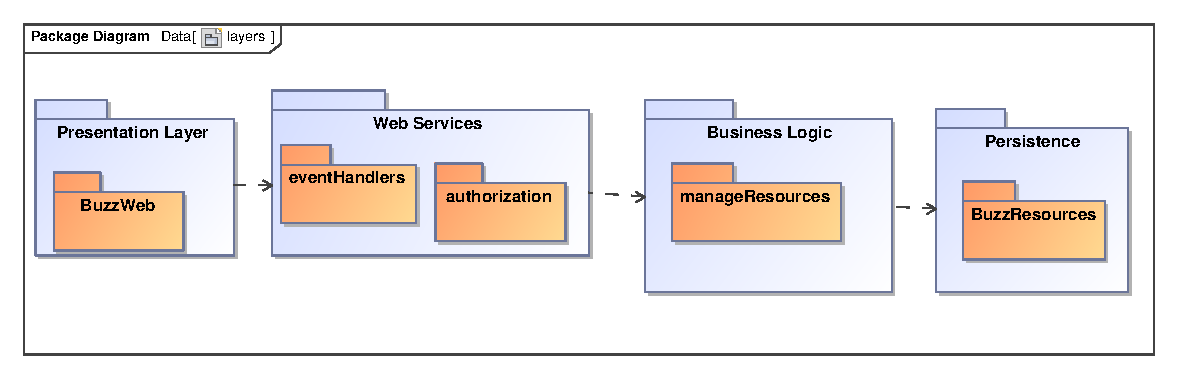
\includegraphics[width=\textwidth]{layers.eps}
\caption{Layering architecture pattern diagram \label{overflow}}
\end{figure}

%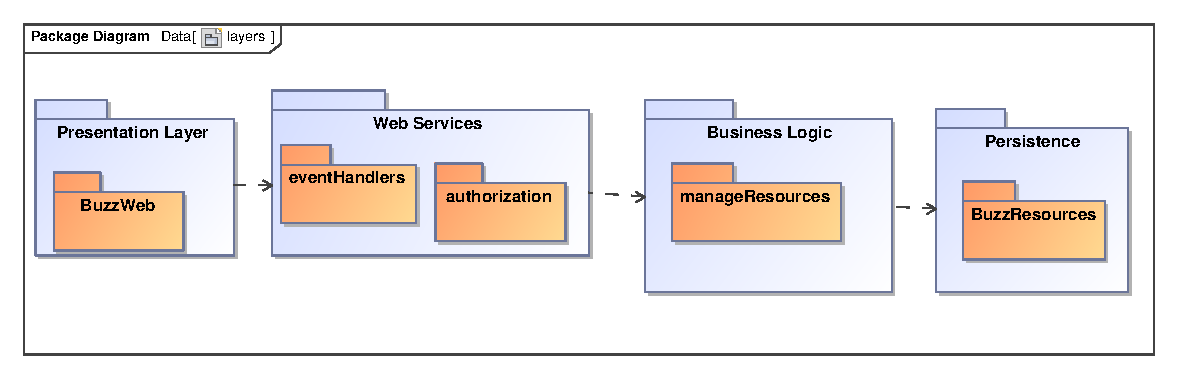
\epsfig{file=layers.eps,width=17cm}

From an MVC perspective:
%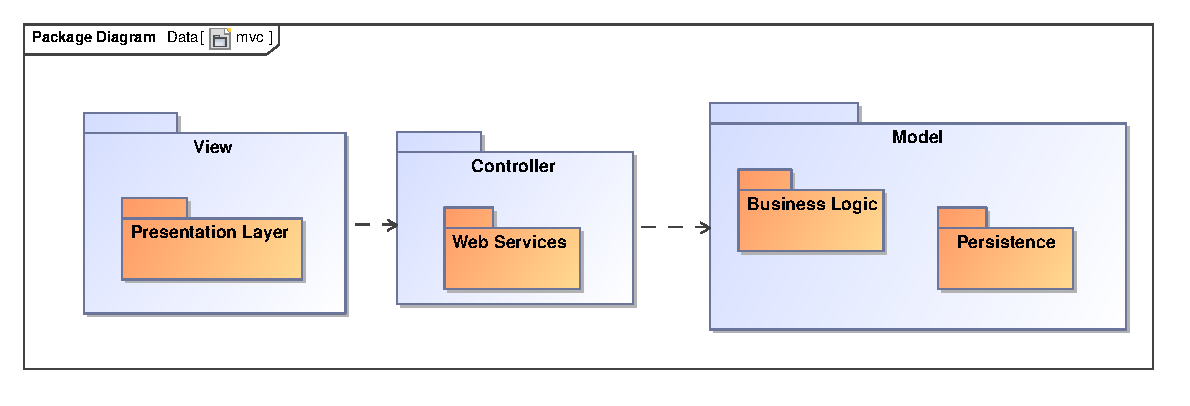
\epsfig{file=mvc.eps,width=17cm}

\begin{figure}[H]                                                                                                                                               
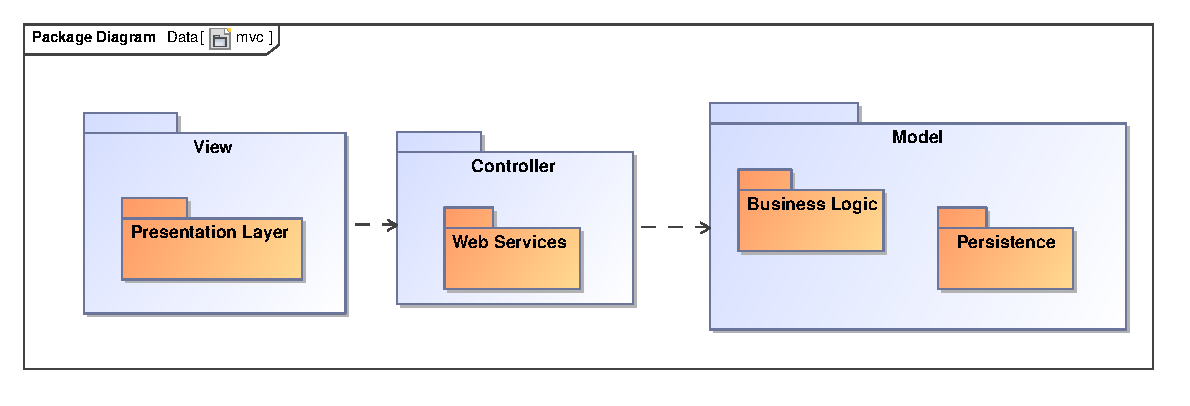
\includegraphics[width=\textwidth]{mvc.eps}
\caption{MVC architecture pattern diagram \label{overflow}}
\end{figure}                                                        
                                                                                                                                                                                                                                                                                                                                                                                                   t
\\
                           
The integration between these layers will be in the form of APIs that each layer will provide to the layer directly above it.
                                                                                                                                      

\subsection{Queueing}
will be using is Queueing. This will help realise the integratability of the system.

\\Queueing is when you queue the different systems' requests to the server in an attempt to allow the server to just focus on one request at a time making it possible to handle requests faster than when it is dividing its attention between multiple requests. By queueing the request any system can send its request and it will be placed into the queue with the other requests. Each system only needs to access the queue, they don't each need remote access to the system. 

\\We will realised this tactic by making use of a queueing system such as FIFO to buffer the server requests until the server is able to handle the next one. 

\\
Using the Layered pattern will improve on the following non-functional requirements:
\begin{itemize}
			\item Pluggability – different services can be tracked easily on the different layers, and can be replaced without compromising the whole system.
			\item Testability – Having different layers will make unit testing very simple since the layers are independent of each other, this implies that mock objects will be used to test each layer.
			\item Maintainability – Different teams can work on the different layers independently and maintain each layer separately.
			\item Security – Having authentication on the presentation layer and authorization in the Web services will increase security because each of these will be localized in one layer, however authentication is mostly left to LDAP.   \\[1em]
\end{itemize}


\section{Architectural Tactics or Strategies}
This section describes the Architectural tactics/strategies which are the conscious design decisions that will influence how the quality requirements are realized in the system. Listed below are the architectural tactics/strategies that we chose to implement in our system as well as which quality requirements they influence and how we plan on implementing them in our system. 
\\
\\\textbf{Course grained services}
\\We will be looking at using course grained services to help realize the performance, scalability, reliability, integrability, reusability, testability and affordability of the system. Coarse grained services is when you group together smaller components and or functions and present it to the user as one big service. This helps with reliability since the users of the system don’t have access to all the smaller private functions, also you can add as many systems as needed since they all will likely just need access to the coarse grained services instead of all the functions the system has to offer.
This strategy will be realized through the construction of the code. Instead of just writing multiple smaller functions we would also write a wrapper functions to encapsulate some of the other functions to make the course grained services. 
\\
\\\textbf{Persistent messaging}
\\The second tactic that we will use is Persistent messaging to help realize scalability, reliability, auditability, integrability, flexibility and maintainability. It also negatively affects performance, affordability and deployment. Persistent messaging is when the messages that are being passed between the systems are sored to disk when send until all the participants have responded that they have received the message. This is done to ensure that the messages will still be delivered even if one of the integration channels breakdown.
This strategy will be realized through the use of a dedicate message broker to facilitate the storage and transfer of messages between the systems. 
\\
\\\textbf{Request/connection dropping}
\\The third tactic that we will be using is Request/connection dropping. This tactic will help to realize scalability, reliability and security. Request/connection dropping is when the connection is closed as soon as the request has been handled in order to lower the network traffic being generated. This allows for more users to use the system at the same time as well as ensures security since if there is no open connections remaining open the risk of someone hacking into a part of the system housing confidential user data is drastically reduces. 
This strategy will be realised through the use of asynchronous threads that close the connection from the client’s side as soon as all the data has been received or from the server’s side if it is going to take a long time to get the data ready for transfer. Then the connection is opened again when the data is ready to be transferred to the client. 
\\
\\\textbf{Run-time}
\\The fourth tactic that we will be using is the run-time tactic. This tactic will help to realize usability. Run-time tactic is when the system is executing and the user gets continuous feedback as to what the system is doing. It gives the user the ability to issue usability commands such as cancel, undo, aggregate and a lot more.  This tactic is both user initiative and system initiative. An example of system initiative is to maintain user or system models
This strategy will be realized through continuous feedback to the user which would improve usability.
\\
\\\textbf{Manage Input/Ouput}
\\Another tactic that we will be using is managing input and output tactic. This tactic will help realize testability in the system. Executing a test requires input to the system and to capture the output. This is called test harness. There are three tactics in which we could manage input and output. The first tactic is record which captures information and uses it as test input. The second tactic is to separate interface from implementation. This allows substitution of implementations for various testing purposes. The last tactic is specialize access to interfaces. There is a hierarchy of test interfaces that can be applied at any level and testing functionality can observe the response of the test.
This strategy will be realized through managing the inputs and outputs of the tests, where input of one component is the output of another component.
\\
\\\textbf{Separation of concerns}
\\The last tactic that we will be using is separation of concerns. This tactic will help realize extensibility, maintainability, reusability and flexibility in the system. This tactic each component is only concerned with only one set of cohesive responsibilities. With this tactic, the system as a whole will become more stable and therefore increase maintainability. The increase in maintainability and extensibility of the system will lead to identifying problems becoming easier and resolution becoming faster.


\section{Use of Reference Architectures and Frameworks}
Reference architectures are often related to software frameworks. Examples of software frameworks include Struts and IBM
Websphere, JBoss aplication server, Microsoft.Net or SeeBeyond.
A framework can thus be defined as a pre-packaged implementation of a reference architecture. It contains actual code and they aim to jump-start application development with a foundation code-base that shapes your architecture and provides utility functions. 
\\\\
We will be making use of Java EE as a reference architecture, the Java Platform, Enterprise Edition architecture is is one of the most widely used reference architectures for large, interactive enterprise systems. The Java Enterprise Edition (JEE) provides a reference architecture within which multi-tier enterprise applications are developed. The specification provides a wide range of standard APIs which must be implemented by Java EE frameworks. But what exactly is a Java EE framework? \textit{It is a tool that can host systems built according to the Java EE reference architecture.}
\\\\
Another widely used reference architecture for enterprise systems is the Services Oriented Architecture (SOA). The Java community has provided a standard API specification for SOA based systems, the Java Business Integration (JBI) specification. SOA provides an infrastructure for defining, maintaining and executing business processes defined across enterprise systems and decoupling enterprise systems such that they just provide services to or request services from the enterprise bus.
\\\\
SOA is not meant to replace Java EE. It does not provide an infrastructure for effectively hosting business logic and does not provide a presentation layer. The individual systems integrated through the enterprise bus may very often be based on the Java EE architecture. So some collaboration between the reference architecture is required for the are trade offs as well as similarities between the two.
\\\\
In any given domain  a Reference Framework  provides a common backplane for consistency, collaboration, sharing, and reuse of the architecture. Without a consistent framework the domain in question will remain an interesting concept but deliver suboptimal business value of the Buzz System. With an appropriate Reference Framework the work of individual projects, programs, divisions and partners will be coordinated with just enough formality to ensure that the many moving parts can fit together when and were needed as to ensure a wholesome and robust system.


\subsubsection{Example Of Architecture Frameworks}
There are many frameworks available which implement this reference \textsl{\textsl{•}}architecture. Some of these are vendor solutions like
\begin{itemize}
\item IBM Websphere
\item BEA WebLogic
\item Oracle Application Server
\end{itemize} 
In addition to these vendor solutions there are also a number of open-source frameworks that realise the Java EE reference architecture, including
\begin{itemize}
\item JBoss,
\item Glassfish,
\item Apache Geronimo, and
\item Jonas.
\end{itemize}
\subsubsection{Why Use Reference Architectures?}
There are many benefits in using reference architectures as a guideline when developing or evaluating the architecture of a work product including:
\begin{itemize}
\item Reduced risk - The reference architecture is bound to address most of the challenges faced by work products for a particular application domain. It is thus less likely that your architecture is inferior due to some oversight.
\item More accessible and hence more maintainable - The reference architecture provides a standard architectural solution for your domain which is bound to be more accessible than some home-grown solution. Maintainability is improved by the reference architecture.
\end{itemize}
\subsubsection{Disadvantages Of Using Reference Architectures}
A disadvantage focusing on using reference architectures is that one might be hindered from coming up with novel solutions which could have provided a competitive edge as now you are fixed to a specific Reference Architecture.


\section{Access and Integration Channels}
The access channel requirements specifies what platforms and technologies are required for the BUZZ System to be accessed by users (desktop computers, laptops). As well as operating systems that the BUZZ system can be accessed on. It also specifies the different networks in which the BUZZ system will use for sending and receiving messages and signals.

\subsubsection{Huamn access channels }
\begin{itemize}
\item The BUZZ system would be made available on platforms like desktop computers, mobile phones, laptops and tablets, it should also be operating systems independent enabling it to be accessed through various operating systems such as  windows, android, iOS, Linux etc. Therefore it can basically be accessed by any device that can connect to the internet since the Buzz system will be hosted on the internet ideally as an add-on to the website of the Department of Computer Science of the University of Pretoria. 
\item The System needs to be able to handle multiple clients logging into the Buzz system at the same time. If there are lets say about 10 000 clients registered on the Buzz system, the system must be constructed in such a way that it can handle all of the clients logging in at the same time. Idealy to help with the traffic, the system needs to be able to host 10 times more clients logging in than what is registered. This will ensure that the operating speed and optimality of the system is of such a state that it would be fast and efficient to use for the clients, ensuring the best service the system can provide.
\item We want our system to be of high standard and quality and therefore the system needs to comply with a few basic standards for example  since it is a web page we will have to validate our page to comply with all HTML 5 standards. 
\item Our system thus also needs to be browser independent to ensure users can access the system not only from any device but also from any browser of their choice making it not only a quality system but also a convenient system.

\item The BUZZ system would need to integrate with various software for example :
\begin{itemize}
\item  MYSQL – To gain access to database functionality to store information for the BUZZ system.
\item JavaScript - To write some functionality and possibly interact with Java programs which will most probably be in charge of activating the sockets and threads and enabling the system to handle multiple users.
\item HTML5 - to construct the web page the system will be hosted on 
\item CSS - to style the Buzz system to not only be user friendly but to also have a ‘nice feel’ to ensure users also enjoy participating on the Buzz system.
\end{itemize}
\end{itemize}

\subsubsection{System access channels }

\begin{itemize}
\item Other systems can access the BUZZ system through the network by gaining access to the  CS(Computer Science) server - cs.up.za. 
\item The server in turn then needs to have access to the database to be able to display all the necessary info stored therein and to ensure only registered users can log in and thus verify their passwords and usernames and then to also allow the system to see the client's privileges and thus allow the client to only perform legal operations when he/she is logged into the Buzz space system and all other database related communications. 
\end{itemize}

\subsubsection{Integration channels }
\begin{itemize}
\item The Buzz System will have to be able to integrate with the University of Pretoria's Department of Computer Science web page, to serve as the Department's discussion forum for all modules and work related topics.  
\item The system needs to be integrated in such a way that if more sub-sections are added and integrated with the system, it will not affect the already existing part or features the system has to offer. 
\item It will however be ideal if the Buzz system can be designed in such a way that it could be used as an add-on to any web page. Thus it needs to be later extended and used on various educational web pages.
\item But for now we just need the Buzz system to integrate with the  University of Pretoria's Computer Science website and thus different requirements needs to be met to enable it to be a safe and quality system. 
\item For example Security aspects needs to comply with that of the Computer Science web page to ensure no harm from students can be done to the web page. Through the Buzz system, any student can have access to the root files of the Buzz system, security measures need to be in place to protect these files.
\item The site also needs to be maintainable and  have a good performance. For example, must be able to handle all students and staff members that can log into the Computer Science web page and more.
\item The system also needs to be flexible, reliable and also user friendly. All these points are more deeply described in the "Quality Requirements" section.
\end{itemize}

\section{Technologies}

\section{References}

\end{document}
